\documentclass[]{article}

\usepackage{hyperref}
\usepackage{graphicx}
\usepackage[margin=0.5in]{geometry}

%opening
\title{Articulate Project \\
Annotation Tools Guide}

\begin{document}

\maketitle

\section{Introduction}
For our annotation purposes, we require just two tools for setup. More details are described in the rest of this document.
\begin{itemize}
	\item ANVIL - video annotation tool
	\item FFmpeg - multimedia conversion tool 
\end{itemize}

\section{FFmpeg Setup}
\subsection{Overview}
Before supplying a video file to ANVIL, it must be converted to H263 codec format. The FFmpeg tool enables us to accomplish this.
\subsection{Installation}
Please click \href{https://www.ffmpeg.org/download.html}{here} and select the appropriate download and then install it.
\subsection{Tutorial}
In order to convert a movie file format, the FFmpeg tool offers command line execution, as described \href{https://www.ffmpeg.org/ffmpeg.html}{here}. For example, the following command converts an ".avi" video to ".mpg": \\\\ 
\fbox{ffmpeg -i source.avi target.mpg}

\subsection{ANVIL Video Format}
The following FFmpeg command-line execution successfully converts video files to an ANVIL-compatible format: \\
\fbox{ffmpeg -i \emph{input.mp4} -vcodec h263 -acodec pcm\_s16be -ac 2 -ar 32000 -s 352x288 -r 25 -ab 32k \emph{output.mov}} \\

\noindent The significance of this command is described below: \\

\noindent \emph{input.mp4}: input file name \\
\emph{output.mov}: output file name. \\
video codec: H263 \\
audio codec: pcm wav, signed 16-bit Big-Endian \\
audio channels: 2 \\
audio sampling frequency: 32000 Hz \\
screen size: 352x288 \\
output frame rate: 25 frames per second \\
output audio bit rate: 32000 bits per second \\

\section{ANVIL Setup}
\subsection{Overview} 
The ANVIL tool assists in video annotation activities. It must be supplied with a coding scheme (referred to as a specification file in ".xml" format) and the video file on which the annotation will be done.

Once the coding scheme and video are supplied to ANVIL, then the user will create a new ".anvil" file and begin annotation. Note that multiple ".anvil" files can be associated to the same coding scheme.

\subsection{Installation}
The ANVIL tool is free and can be downloaded and installed by following the instructions \href{http://www.anvil-software.org/download/index.html}{here}

\subsection{Tutorial}
Once installed, the next step is to become familiar with use of the tool. Fortunately, tutorial videos have already been created for this purpose and can be viewed by clicking \href{http://www.anvil-software.org}{here} followed by clicking on the "Video Tutorials" link. 

Note that the video referring to "Transcribing speech with PRAAT" can be ignored (we will not be using it for our annotations).

\subsection{Articulate Coding Scheme}
The Articulate coding scheme is available at bitbucket: \\ git@bitbucket.org:articulateannotations/annotations.git

\section{Example}
Once ANVIL and FFmpeg are setup, the following is a step-by-step guide of a successful annotation of subject 11 from the Articulate user study.

\begin{enumerate}
\item Convert incompatible user study video file using FFmpeg: \\
\fbox{ffmpeg -i back.mp4 -vcodec h263 -acodec pcm\_s16be -ac 2 -ar 32000 -s 352x288 -r 25 -ab 32k subject11.mov} \\

\item Select "subject11.mov" video file in ANVIL. \\
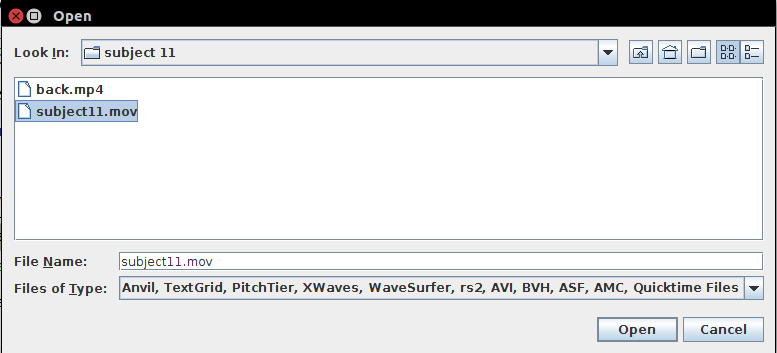
\includegraphics[width=0.5\textwidth]{choose_video_file.png}

\item Select the coding scheme specification file "ArticulateStudySpecification1.xml" obtained using bitbucket. \\
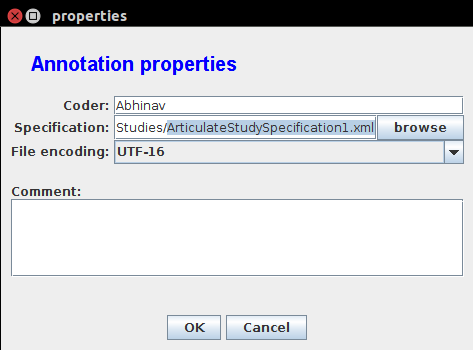
\includegraphics[width=0.5\textwidth]{choose_coding_scheme.png}

\item Save the ".anvil" file, which stores reference to coding scheme file, annotations made, and selected video file. \\
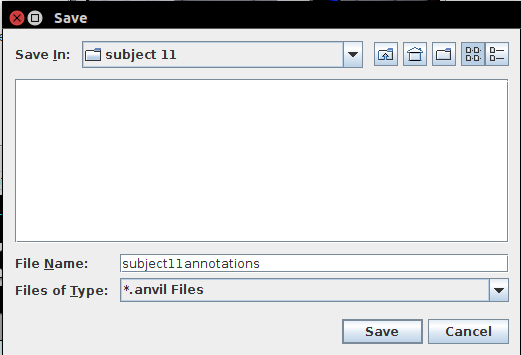
\includegraphics[width=0.5\textwidth]{save_annotations_file.png}

\item Under the Annotations tracks, select the "Questions" track in the range 07:46 to 07:51. Then, right-click and select "Create \& Edit" menu option.

\item Enter "Q1" for QuestionID and "Let's start with the activity around UIC?" for Transcription. \\
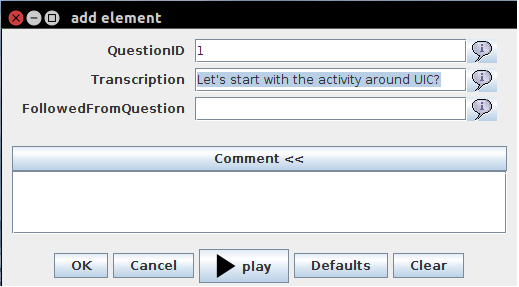
\includegraphics[width=0.5\textwidth]{add_transcription_element.png}
\\
\item The first question has been successfully annotated for subject 11.
\end{enumerate}

\end{document}
